\begin{example}
	\index{Example: HMC Hamiltonian variable change}
	Let $\xi \equiv e^\zeta$, such that $\zeta\in [-\infty,\infty]$ maps to $\xi\in[0,\infty]$ and $\xi$ is ensured to be positive definite regardless of the value of $\zeta$. Using the differential $d\xi =  \xi d\zeta$ in equation \eqref{eq:q3} means $p(\theta,\xi,\lambda|D,I)$ is multiplied with $\xi$. Hence, when taking $-\ln(p(\theta,\xi,\lambda|D,I))$ according to equation \eqref{eqh}, a $-\ln(\xi)$ is added to the Hamiltonian. In practice this means
	\begin{equation}
		(1-\tilde{\alpha})\ln(\xi)\in H\Rightarrow -\tilde{\alpha}\ln(\xi).
	\end{equation} 	
\end{example}

\begin{example}
	\begin{equation}
		C(U(x), s) = \alpha\cdot \text{swish}(U(x)-s,\beta)+(1-\alpha)\cdot\text{swish}(s-U(x),\beta)
	\end{equation}
	where
	\begin{equation}
		\text{swish}(z,\beta) = \frac{z}{1+e^{-z\beta}}.
	\end{equation}
	and $z\equiv U(x)-s$. Taking $\alpha \ll 1$, then $z<0$ will be penalized relatively more than $z>0$. $z<0$ corresponds to underestimation, so this is penalized greater relative to overestimation. Now
	\begin{equation}
		\begin{split}
			\mathbb{E}[C|\dots ] & =\int ds p(s|\dots) \bigg(\alpha\cdot \text{swish}(U(x)-s,\beta)+(1-\alpha)\cdot\text{swish}(s-U(x),\beta)\bigg)
		\end{split}
	\end{equation}
	Let $z\equiv U(x)-s$, then
	\begin{equation}
		\begin{split}
			\frac{dC}{dU(x)} & = \frac{dC}{dz}\frac{dz}{dU(x)}\\
			& = \bigg(\frac{\alpha}{1+e^{-\beta z}}-\frac{1-\alpha}{1+e^{\beta z}}+\frac{\alpha\beta e^{-\beta z}z}{(1+e^{-\beta z})^2}+\frac{(1-\alpha)\beta e^{\beta z}z}{(1+e^{\beta z})^2}\bigg)\frac{dz}{dU(x)}\\
			&= \frac{\beta z e^{\beta z}-e^{\beta z}-1}{(1+e^{\beta z})^2}+\alpha+\mathcal{O}(\alpha^2)\\
			&\approx  \alpha -\frac{1}{(1+e^{\beta z})^2}
		\end{split}
	\end{equation}
	\begin{equation}
		\begin{split}
			\frac{d\mathbb{E}[C|\dots ]}{dU(x)} &\approx \int ds p(s|\dots) \bigg(\alpha -\frac{1}{(1+e^{\beta z})^2}\bigg)\\
			& = \alpha -\int ds p(s|\dots)\frac{1}{(1+e^{\beta z})^2}\\
			& = 0
		\end{split}
	\end{equation}
	$\frac{1}{(1+e^{\beta z})^2}$ approximate a unit step which is $1$ for $z<0$ and $0$ otherwise. $z<0 \Rightarrow s>U(x)$. This means
	\begin{equation}
		\int_{-\infty}^{\infty} ds p(s|\dots)\frac{1}{(1+e^{\beta z})^2} \approx \int_{U(x)}^{\infty} ds p(s|\dots)
	\end{equation}
	This means
	\begin{equation}
		\alpha \approx \int_{U(x)}^{\infty} ds p(s|\dots)
	\end{equation}
\end{example}

\begin{example}
	Suppose there is a game between a Robot and Nature in which the Robot objective is to guess the position of the Robot. The Robot is given measurements of its velocity and acceleration, at any time step and must formulate a belief about its position. Nature decides the true position of the Robot and will penalize the Robot according to the deviation between the Robots estimate of its position and the true position viz
	\begin{equation}
		C(U(x),s) = (U(x)-s)^2,
	\end{equation}
	where $s$ is the true position $U(x)$ is the Robots estimate based on data $x$ containing velocity and acceleration measurements. 
	\begin{figure}[H]
		\centering
		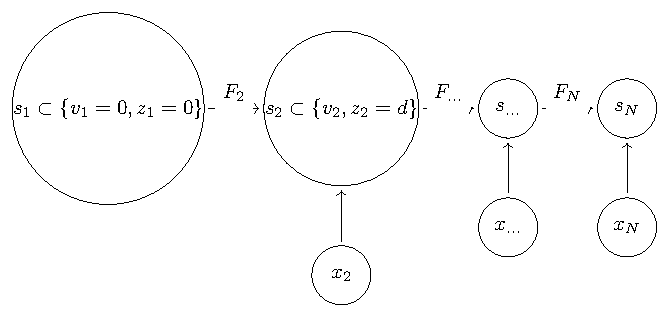
\includegraphics[width = 0.5\textwidth]{figures/graph.pdf}
		\caption{}
		\label{fig:1}
	\end{figure}
	Suppose the Robot is given all historical data, then the expected cost can be written
	\begin{equation}
		\mathbb{E}_{S|X}[C(U(X),S|s_1,\{x\}_{2:N},I)] = \int ds (U(x_N)-s)^2p(s|s_1,\{x\}_{2:N},I).
	\end{equation}
	The optimal decision is defined by
	\begin{equation}
		\frac{d}{dU(X)}\bigg(\mathbb{E}_{S|X}[C(U(X),S|s_1,\{x\}_{2:N},I)]\bigg)\bigg|_{U(x_N)=U^*(x_N)} = 0
	\end{equation}
	leading to 
	\begin{equation}
		U^*(x_N) = \mathbb{E}[S_{N}|s_1,\{x\}_{2:N},I].
		\label{eq:dr}
	\end{equation}
	The inutitive interpretation of equation \eqref{eq:dr} is that the optimal decision of the Robot is to estimate the position that it expects Nature to have chosen. Now
	\begin{equation}
		\mathbb{E}[S_{N}|s_1,\{x\}_{2:N},I] = \int ds_{N} s_N p(s_N|s_1,\{x\}_{2:N},I).
		\label{eq:a5}
	\end{equation}
	Assume that
	\begin{equation}
		\begin{split}
			p(s_i|s_{i-1},I) &= N(s_i|\mu_i = F_is_{i-1}+b_i,\Sigma_i = Q_i),\\
			p(x_i|s_{i},I) &= N(x_i|\mu_i = H_is_{i}+d_i,\Sigma_i = R_i)
		\end{split}
		\label{eq:a2}
	\end{equation}
	Hence, $p(s_N|s_1,\{x\}_{2:N},I)$ must be reformulated such that the above can be utilized. 
	Now
	\begin{equation}
		\begin{split}
			p(s_N|s_1,\{x\}_{2:N},I) &= \frac{p(x_{N}|s_N,s_1,\{x\}_{2:N-1},I)p(s_N|s_1,\{x\}_{2:N-1},I)}{p(x_{N}|s_1,\{x\}_{2:N-1},I)}\\
			&= \frac{p(x_{N}|s_N,I)p(s_N|s_1,\{x\}_{2:N-1},I)}{p(x_{N}|s_1,\{x\}_{2:N-1},I)}\\
		\end{split}
		\label{eq:a3}
	\end{equation}
	where
	\begin{equation}
		\begin{split}
			p(s_N|s_1,\{x\}_{2:N-1},I) &= \int ds_{N-1}p(s_N,s_{N-1}|s_1,\{x\}_{2:N-1},I)\\
			&= \int ds_{N-1}p(s_N|s_{N-1},s_1,\{x\}_{2:N},I)p(s_{N-1}|s_1,\{x\}_{2:N-1},I)\\
			&= \int ds_{N-1}p(s_N|s_{N-1})p(s_{N-1}|s_1,\{x\}_{2:N-1},I)\\
			&= \int ds_{N-1} N(s_{N}|F_{N}s_{N-1}+b_{N},Q_{N})N(s_{N-1}|\mu_{N-1},\Sigma_{N-1})\\
			&=N(s_{N}|\mu_{N|N-1},\Sigma_{N|N-1})
		\end{split}
		\label{eq:a1}
	\end{equation}
	where 
	\begin{equation}
		\begin{split}
			\mu_{N|N-1} &= F_{N}\mu_{N-1}+b_N\\
			\Sigma_{N|N-1} &= F_{N}\Sigma_{N-1}F_{N}^T+Q_{N}\\
		\end{split}
	\end{equation}
	Using equation \eqref{eq:a1} and \eqref{eq:a2} in equation \eqref{eq:a3} then yields~\citep{murphy2023probabilistic}
	\begin{equation}
		p(s_N|s_1,\{x\}_{2:N},I) = N(s_N|\mu_{N},\Sigma_N)
		\label{eq:a4}
	\end{equation}
	where
	\begin{equation}
		\begin{split}
			\mu_{N} &= \mu_{N|N-1}+K_N(x_N-\hat{x}_N),\\
			\Sigma_{N} &= \Sigma_{N|N-1}-K_NS_NK_N^T,\\
			K_N & = \Sigma_{N|N-1}H_N^TS_N^{-1},\\
			\hat{x}_N&= H_N\mu_{N|N-1}+d_N,\\
			S_N & = H_N\Sigma_{N|N-1}H_N^T+R_N\\
		\end{split}
	\end{equation}
	Combining equation \eqref{eq:a4} with \eqref{eq:a5} then yields the optimal decision for the Robot
	\begin{equation}
		\mathbb{E}[S_{N}|s_1,\{x\}_{2:N},I] = \mu_{N}.
	\end{equation}
	
\end{example}

\begin{example}
	Consider a Robot moving in one dimension. Every time interval $\Delta t$, the Robot will sample a wheel counter and an accelerometer. The wheel counter will be incremented every distance $d$. The Robot is interested in knowing its position and velocity. Expand the position viz
	\begin{equation}
		z(t+\Delta t)=z(t)+\Delta t \frac{dz(t)}{dt}+\frac{1}{2}(\Delta t)^2\frac{d^2z(t)}{dt^2}+\mathcal{O}(\Delta t^3)
	\end{equation}
	which discretize to
	\begin{equation}
		z_k\simeq z_{k-1}+\Delta t v_{k-1}+\frac{1}{2}(\Delta t)^2a_{k-1},
	\end{equation}
	where $\Delta t = \text{const}$ and
	\begin{equation}
		\begin{split}
			v_k &\simeq v_{k-1}+\Delta t a_{k-1},\\
			a_k &\simeq a_{k-1},
		\end{split}
	\end{equation}
	This means
	\begin{equation}
		\begin{split}
			s_k &= \begin{pmatrix}
				z_k\\ v_{k} \\ a_k\\
			\end{pmatrix}\\
			& \simeq \underbrace{\begin{pmatrix}
					1 & \Delta t & \frac{1}{2}\Delta t^2  \\
					0 & 1 & \Delta t  \\
					0 & 0 & 1  \\
			\end{pmatrix}}_{=F_k}\begin{pmatrix}
				z_{k-1}\\ v_{k-1} \\ a_{k-1}\\
			\end{pmatrix}
		\end{split}
	\end{equation}
	where $b_k=\emptyset$ for simplicity. Now take
	\begin{equation}
		\begin{split}
			x_k &= \begin{pmatrix}
				c_k \\ a_k
			\end{pmatrix}\\
			&= \underbrace{\begin{pmatrix}
					d^{-1} & 0 & 0\\
					0 & 0 & 1 
			\end{pmatrix}}_{=H_k}\begin{pmatrix}
				z_{k-1}\\ v_{k-1} \\ a_{k-1}\\
			\end{pmatrix}+r_k
		\end{split}
	\end{equation}
	where $r_k \sim N(0,R_k)$ with 
	\begin{equation}
		R_k = \begin{pmatrix}
			\sigma_z^2 & \sigma_z\sigma_a\\
			\sigma_z\sigma_a & \sigma_a^2 \\
		\end{pmatrix},
	\end{equation}
	where $\sigma_z$ and $\sigma_a$ are estimated from observations. The process noise can be determined viz~\href{https://github.com/rlabbe/Kalman-and-Bayesian-Filters-in-Python/blob/master/07-Kalman-Filter-Math.ipynb}{Kalman link}
	\begin{equation}
		Q_k = \begin{pmatrix}
			\frac{\Delta t^4}{4} & \frac{\Delta t^3}{2} & \frac{\Delta t^2}{2}\\
			\frac{\Delta t^3}{2} & \Delta t^2 & \Delta t\\
			\frac{\Delta t^2}{2} & \Delta t & 1\\
		\end{pmatrix}\sigma^2,
	\end{equation}
	where $\sigma \sim \Delta a$.
\end{example}


\begin{example}

	 Specifically, a first attempt at quantifying what is called \emph{Renzo's rule}~\cite{Renzosrule} by using Bayesian artificial neural networks (BANNs) to detect anomalies in the baryonic and observed galactic rotation curves will be presented. Renzo's rule state that\newline
	
	\emph{"every time there is a feature in the radial light distribution the rotation curve shows a corresponding feature"}\newline
	
	It has been corroborated by examining the quality of fits from scaling the contributions of baryonic matter in rotation curves~\cite{Swaters2010,Swaters2012,Famaey2012} and is sometimes used as an argument in favor of modified gravitational dynamics (see e.g. \cite{Swaters2010,Famaey2012}).\newline 
	The basic idea for quantifying Renzo's rule is to let two separate BANNs identify anomalies in the baryonic and observed galactic rotation curves such that the coincidence of the anomalies can be compared and analyzed. In theory, if Renzo's rule is completely accurate and the anomalies detected by the BANNs correspond to features in the baryonic and observed rotation curves, one would expect a one-to-one correspondence between the anomalies in the baryonic and observed rotation curves. Due to measurement imperfections in the independent measurements techniques of the baryonic and observed rotation curves, it is, however, not expected that there be a complete one-to-one correspondence even if Renzo's rule is completely accurate and the anomalies detected by the BANNs correspond to features in the baryonic and observed rotation curves. However the method presented and the initial results motivate further investigation. 
	
	\section{Data}
	Data from the SPARC database with selection criteria identical to Paper III~\cite{Petersen:2017klw} is used in Paper VI~\cite{Petersen:2020renzo}. This means rotation curve data from $152$ galaxies making up $3143$ rotation curve points.
	
	\section{Considerations regarding approach}
	In order to quantify Renzo's rule, the degree of coincidence of anomalies in the baryonic rotation curve, $v_{bar}(r)$, and the observed rotation curve, $v_{obs}(r)$, will be investigated in this study. In order to quantify anomalies as objectively and unbiased as possible, two autoencoder (AE) BANNs will be used -- One (AE$_{obs}$) with input $\{r,v_{obs}\}$ and the other (AE$_{bar}$) with input $\{r,v_{bar}\}$. The autoencoder will construct a representation of the input and transform the input back and forth between the representation. After successful training on a set of training data, the autoencoder will be able to reconstruct test input that is similar to that of the training input. In order to test Renzo's rule as accurately as possible, it is desired that the autoencoder is trained on featureless data such that it will raise a metaphorical flag every time it encounters a feature in the test data. In order to avoid the bias associated with cherry picking featureless data for training, a set of $152$ mock galaxies are generated using randomly perturbed parameters from the SPARC galaxies (to ensure the parameters used are different but realistic). This is done by sampling an exponential disk profile~\cite{binney} with noise corresponding to a $5\%$ relative uncertainty
	\begin{equation}
		v_{bar}^{(mock)} \sim \mathcal{N}(v_N,0.05v_N),
		\label{vbar}
	\end{equation}
	where in equation \eqref{vbar} "$\sim$" denote "distributed as" and
	\begin{equation}
		v_N= \sqrt{\frac{G_Nm_dr^2}{2r_d^3}\bigg(I_{0}\bigg(\frac{r}{2r_d}\bigg)K_{0}\bigg(\frac{r}{2r_d}\bigg)-I_{1}\bigg(\frac{r}{2r_d}\bigg)K_{1}\bigg(\frac{r}{2r_d}\bigg)\bigg)}
		\label{vn}
	\end{equation}
	with $G_N$ being Newtons gravitational constant,  $m_d=2\pi r_d^2\Upsilon^{d} S_d$ the central surface density with the disc mass to light ratio $\Upsilon^{d}=0.5\frac{m_\odot}{L_\odot}$~\cite{Lelli:2017vgz}. $S_d$ and $r_d$ is determined by randomly perturbing the corresponding measured quantities of the SPARC database. The exponential disk profile is sampled in the range $\{0,10\}r_d$ with $50$ data points. The mock data for $v_{obs}$ is generated using the Radial Acceleration Relation (RAR)~\cite{McGaugh:2016leg} such that
	\begin{equation}
		v_{obs}^{(mock)} \sim \mathcal{N}(v_{tot},0.05v_{tot}),
		\label{vobs}
	\end{equation}  
	where in equation \eqref{vobs} "$\sim$" denote "distributed as" and
	\begin{equation}
		v_{tot}=v_N \bigg(1-e^{-\sqrt{\frac{v_N^2}{a_0r}}}\bigg)^{-\frac{1}{2}}
		\label{vtot}
	\end{equation}
	with $a_0=1.2\cdot 10^{-10}\frac{m}{s^2}$. Using the training data from the $152$ mock galaxies, a feature is defined as \emph{the input the AE -- trained on featureless mock galaxies -- is not able to reconstruct accurately}. What constitutes "accurately" will be elaborated later on.\newline
	
	To keep things simple, both AEs will be on the form of two-layer perceptrons~\cite{hastie_09,murphy2013machine} with sigmoid activation functions, meaning 
	\begin{equation}
		\begin{split}
			f_k^{(n)}&=b_k^{(3)}+\sum_{l=1}^{n_2}W_{kl}^{(3)}h_{l}^{(n,2)},\\
			h_{l}^{(n,2)}&=g\bigg(b_l^{(2)}+\sum_{m=1}^{n_1}W_{lm}^{(2)}h_{m}^{(n,1)}\bigg),\\
			h_{m}^{(n,1)}&=g\bigg(b_m^{(1)}+\sum_{s=1}^{P}W_{ms}^{(1)}x_{s}^{(n)}\bigg),
		\end{split}
		\label{n2}
	\end{equation}
	where $b,W$ are coefficients (collectively denoted by $\theta$), $K = P$ for an AE and
	\begin{equation}
		\begin{split}
			g(z)&=\text{sig}(z)\\
			&=\frac{1}{1+e^{-z}}.
		\end{split}
	\end{equation}
	This choice of $g$ shrink the influence of lower level coefficients since
	\begin{equation}
		\begin{split}
			\frac{d \text{sig}(z_j)}{d z_u}&=\text{sig}(z_j)(1-\text{sig}(z_j))\delta_{ju}\\
			&\lesssim \frac{1}{4}
		\end{split}
	\end{equation}
	will be contained in the gradients used for training. This is the so-called "vanishing gradients problem"~\cite{Bengio1994,Bengio1995}. By training the AE via Hamiltonian Monte Carlo (HMC)~\cite{Duane:1987de,Neal:1996,Neal2012}, the problem can be alleviated to some degree for small $z$ by adjusting the parameters of the algorithm (the masses). In order for $z$ to be small, the input must be normalized. Due to the lack of normality of the input data (the rotation curve data), data is normalized according to
	\begin{equation}
		\begin{split}
			\{\breve{r},\breve{v}_{bar}\} &\equiv \bigg\{\frac{r-\min(r)}{\max(r)-\min(r)},\frac{v_{bar}-\min(v_{bar})}{\max(v_{bar})-\min(v_{bar})}\bigg\},\\
			\{\breve{r},\breve{v}_{obs}\} &\equiv \bigg\{\frac{r-\min(r)}{\max(r)-\min(r)},\frac{v_{obs}-\min(v_{obs})}{\max(v_{obs})-\min(v_{obs})}\bigg\},
		\end{split}
	\end{equation}
	where the $\max$ and $\min$ operations go over all data points in the training/test data, respectively. The normalized radii and velocities for the test and training data are shown in figure \ref{fig:data} in appendix \ref{app:figs}. The $\min$ and $\max$ operations are non-differentiable, which means the systematic uncertainties included in the variables (inclination, $\alpha$, distance, $D$, and the unitless mass to light ratios $\tilde{\Upsilon}$) cannot be marginalized over -- as would otherwise be an obvious choice in the Bayesian formalism. Instead, the uncertainties of the input data are treated as hyper parameters, $\xi$, controlled by a set of vague priors in order to be as unbiased as possible. Due to the treatment of the uncertainties the data from different galaxies can be stacked "head to tail" in the input array, $x^{(n)}_k$, with $k$ referring to the input variables and $n$ the data entry. The target values, $y_k^{(n)}$, are equal to the input ($y_k^{(n)}=x_k^{(n)}$) for the AE, but to avoid confusion the notational distinction between the two are kept. In order for the AE to be able to detect structure in the rotation curves, the AE take $5$ consecutive rotation curve points as input, meaning $k=1,2,\dots 10$ (since the input consists of $5$ radial points and $5$ velocity points) and $n=1,2,\dots3138$ (note the endpoint is $3143-5$) for the test data. 
	
	\section{Method}
	The idea is to feed $v_N$ to a two-layer perceptron and fit it to $v_N$ (an auto encoder). Then after this, the auto encoder will be fed $v_{bar}$ and it when behavior that deviates from the theoretical one is encountered, the model will flag this. This is done for both the baryonic and observed curved. Then the positioning of anomalies can be compared.
	
	Perhaps we can do this more directly? In the end I consider the expectation of $c_3$ under two different assumptions.. I could compute this directly, or perhaps it is more fitting to consider some variant of the bayes factor here? 
	
	The disadvantage of the approach with auto-encorders is that generally unfamiliar data is labeled as anomalies.
	
	
	\section{Analysis}
	Each AE ($\text{AE}_{obs}$ and $\text{AE}_{bar}$) are trained for $5000$ iterations on the rotation curve data from the $152$ mock galaxies. Figure \ref{fig:energy} in appendix \ref{app:figs} show the Hamiltonian for each AE as a function of iterations. As is evident figure \ref{fig:energy}, convergence to the stationary distribution is achieved around iteration $\approx 950$. To be conservative, the first $1000$ iterations of each training is treated as burn in. To measure the accuracy with which the AE's can reproduce the input the average residual squared per output, $\zeta$, is considered  
	\begin{equation}
		\zeta^{(i)}\equiv\frac{1}{K}\sum_{k=1}^{K}\bigg(\frac{1}{N_{p_8}}\sum_{q\in p_8}\xi_{k,q}(f_k(x^{(i)},\theta_q)-y^{(i)}_k)\bigg)^2,
		\label{R}
	\end{equation}
	with $N_{p_8}=4000$ (i.e. the $5000$ iterations minus burn in). $\zeta^{(i)}$ is a measure similar to the chi square per test data point. Figure \ref{fig:R} in appendix \ref{app:figs} show $\zeta^{(i)}$ for the test data. The goal is to identify instances for which the input is reproduced less well and analyze the correspondence between $\text{AE}_{obs}$ and $\text{AE}_{bar}$ for these instances. For this reason, an anomaly is defined as $\zeta^{(i)}> A$, with $A$ being a threshold. Associated with the anomalies three different counters of anomalies are defined
	\begin{enumerate}
		\item $C_1$ the number of instances, $i$, for which an anomaly is only detected in $\text{AE}_{bar}$ (i.e. $\zeta_{\text{AE}_{obs}}^{(i)}<A\wedge \zeta_{\text{AE}_{bar}}^{(i)}>A$).
		\item $C_2$ the number of instances, $i$, for which an anomaly is only detected in $\text{AE}_{obs}$ (i.e. $\zeta_{\text{AE}_{obs}}^{(i)}>A\wedge \zeta_{\text{AE}_{bar}}^{(i)}<A$). 
		\item $C_3$ the number of instances, $i$, for which an anomaly is detected in both $\text{AE}_{bar}$ and $\text{AE}_{obs}$ (i.e. $\zeta_{\text{AE}_{obs}}^{(i)}>A\wedge \zeta_{\text{AE}_{bar}}^{(i)}>A$).  
	\end{enumerate}
	From the definitions of $C_1,C_2$ and $C_3$, the fraction of anomalies corresponding to $C_1,C_2$ and $C_3$ are defined viz
	\begin{equation}
		\begin{split}
			c_1 &\equiv \frac{C_1}{C_1+C_2+C_3},\\
			c_2 &\equiv \frac{C_2}{C_1+C_2+C_3},\\
			c_3 &\equiv \frac{C_3}{C_1+C_2+C_3}.\\
		\end{split}
	\end{equation}
	In relation to Renzo's rule, $c_3$ -- the fraction of anomalies that appear in both the baryonic and observed rotation curves -- is of particular interest, since in the case where Renzo's rule is completely accurate and the anomalies detected by the AE's correspond to features in the baryonic and observed rotation curves, $c_3=1$ and $c_1=c_2=0$. Figure \ref{fig:res} show the measured $c_1,c_2$ and $c_3$ as function of $A$ for the test data (SPARC galaxies). A small sanity check is that when $A=0$ everything is counted as anomalies and hence $c_3=1$ by definition. Because $\zeta$ can be interpreted as a measure similar to chi-square per degree of freedom $A=1$ loosely translates to counting the points that are anomalous with more than $1$ sigma. For $A\simeq 1$
	\begin{equation}
		c_1\approx 0.2, \qquad c_2\approx 0.4, \qquad c_3\approx 0.4.
		\label{res}
	\end{equation}
	In order to interpret the values of $c_3$ from figure $\ref{fig:res}$, it is expedient to consider a rough reference point; the expected value of $c_3$ can roughly be represented as
	\begin{equation}
		\mathbb{E}[c_3]\approx\frac{1}{N_{test}}\sum_{i=1}^{N_{test}}\frac{\mathbb{P}_1^{(i)}}{\mathbb{P}_2^{(i)}}.
		\label{P3}
	\end{equation}
	with $N_{test} = 3138$ being the number of test points, $\mathbb{P}_1^{(i)}$ the probability of simultaneous anomalies and $\mathbb{P}_2^{(i)}$ the probability of an anomaly. Formally
	\begin{equation}
		\begin{split}
			\mathbb{P}^{(i)}_1&=\mathbb{P}(\zeta^{(i)}_{obs}>A,\zeta^{(i)}_{bar}>A|x^{(i)},\xi,\theta,I),\\
			\mathbb{P}^{(i)}_2& = \mathbb{P}_3^{(i)}+\mathbb{P}_4^{(i)}-\mathbb{P}_1^{(i)},\\
		\end{split}
		\label{eq1a}
	\end{equation}
	with
	\begin{equation}
		\begin{split}
			\mathbb{P}_3^{(i)}& \equiv\mathbb{P}(\zeta^{(i)}_{obs}>A|x^{(i)},\xi,\theta,I),\\
			\mathbb{P}_4^{(i)}& \equiv\mathbb{P}(\zeta^{(i)}_{bar}>A|x^{(i)},\xi,\theta,I).
		\end{split}
	\end{equation}
	If the anomalies in the baryonic and observed rotation curves are independent then 
	\begin{equation}
		\mathbb{P}_1^{(i)} = \mathbb{P}_3^{(i)}\mathbb{P}_4^{(i)}.
		\label{P2}
	\end{equation}
	Assuming for simplicity that there is no correlation between different anomalous data points in the observed rotation curve and different anomalous data points in the baryonic rotation curve, then
	\begin{equation}
		\begin{split}
			\mathbb{P}_3^{(i)}\approx  \frac{n_{ano}^{(obs)}}{N_{test}}, \qquad
			\mathbb{P}_4^{(i)}\approx \frac{n_{ano}^{(bar)}}{N_{test}}.
		\end{split}
		\label{P1}
	\end{equation}
	with $n_{ano}^{(obs)}$ being the number of test points for which $\zeta^{(i)}_{obs}>A$ and $n_{ano}^{(bar)}$ being the number of test points for which $\zeta^{(i)}_{bar}>A$. Combining equations \eqref{P3}-\eqref{P1} yield
	\begin{equation}
		\mathbb{E}[c_3]\approx\frac{n_{ano}^{(obs)}n_{ano}^{(bar)}}{N_{test}\left(n_{ano}^{(obs)}+n_{ano}^{(obs)}-\frac{n_{ano}^{(obs)}n_{ano}^{(bar)}}{N_{test}}\right)}.
		\label{P4}
	\end{equation}
	The result is displayed as the black line in figure \ref{fig:res}. 
	\begin{figure}[ht]
		\centering
		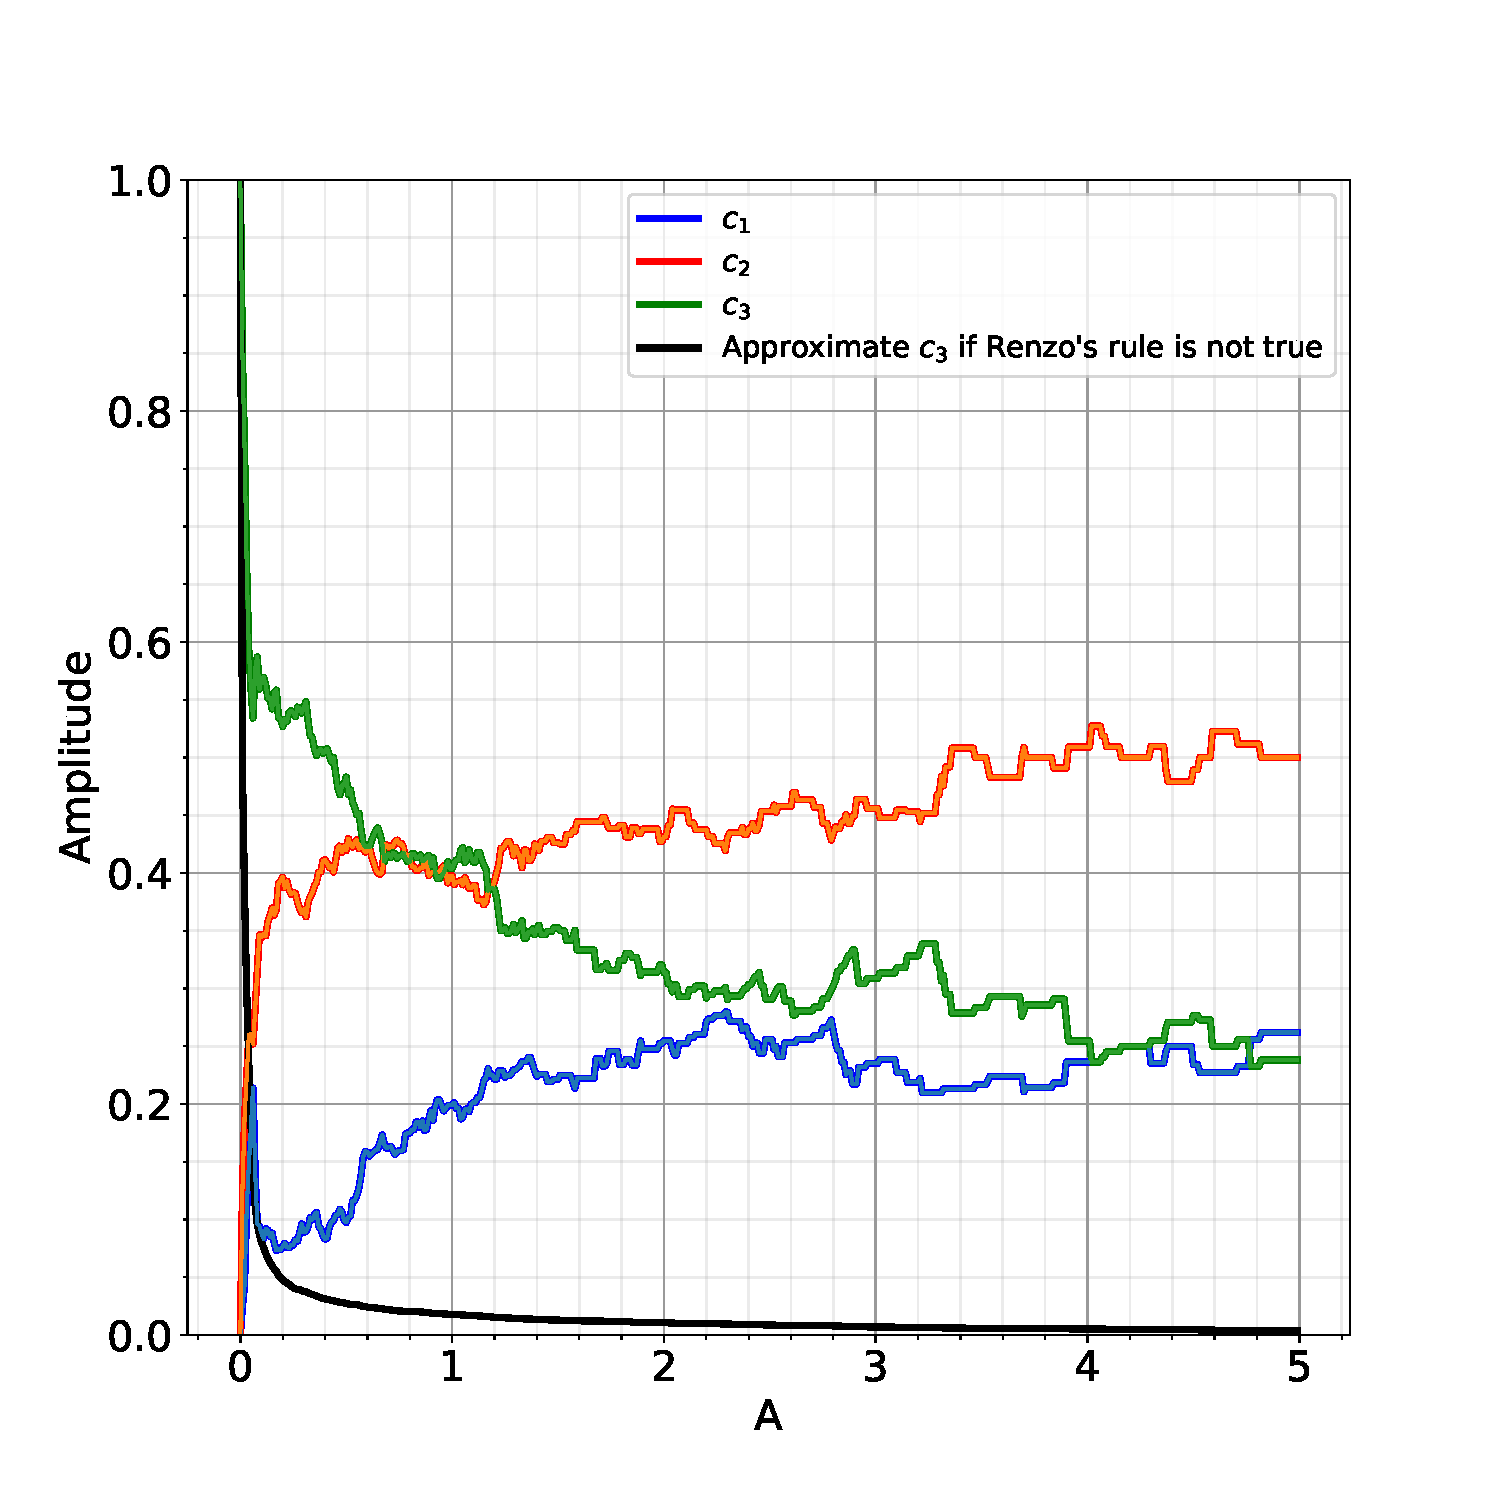
\includegraphics[width=1\textwidth]{figures/res.pdf}
		\caption{$c_1$ (blue), $c_2$ (orange) and $c_3$ (green) as a function of the threshold for detection, $A$, for the test data (SPARC galaxies). Reproduction of figure 1 from Paper VI~\cite{Petersen:2020renzo}.}
		\label{fig:res}
	\end{figure}
	In the figure the green line show the fraction of anomalous points that are coincident, $c_3$, in the two AE's as a function of the threshold used to define an anomaly, $A$. As stated previously, in an idealized setting with perfect data and method, Renzo's rule predicts $c_3=1$ for all $A$. However, because of i) measurement imperfections in the independent measurements techniques of the baryonic and observed rotation curves and ii) a non-perfect correspondence between anomalies detected by the BANNs and features that may be subjectively defined (see appendix \ref{ch:disc} for an extended discussion on this topic), $0<c_3<1$ is expected for $A>0$ even if Renzo's rule is completely accurate. The black curve in figure \ref{fig:res} show the value of $c_3$ that is naively expected if anomalies in the baryonic and observed rotation curves are random and hence Renzo's rule is not true. Comparing the green and black curves from figure \ref{fig:res}, it is clear that -- although it is not possible to determine an exact expected value for $c_3$ in case Renzo's rule is true -- within the simplified setting considered, correlations between anomalies in the baryonic and observed rotation curves that are significantly higher than random  are found-- as required by Renzo's rule. When an anomaly is present in either the baryonic or observed rotation curve, the anomaly is coincident (i.e. an anomaly is detected in both rotation curves at the same instance) in about $40\%$ of instances. Figures \ref{fig:rot}-\ref{fig:rot4} in appendix \ref{app:figs} show rotation curves for all the galaxies with detected anomalies using $A=1$. Reviewing the detected anomalies it is clear that coincident anomalies are abundant at all radii.
	
	
\end{example}